\chapter{Results on means and tools for primary tool chain}
\label{sec:results}

\section{Initial  list of candidates}

The initial list of candidates is the following:


\begin{enumerate}

\item  GOPRR
\item  CORE
\item  ERTMSFormalSpecs
\item  SysML with Papyrus
\item  SysML with Entreprise Architect
\item  SCADE
\item  EventB with Rodin
\item  Classical B with Atelier B
\item  Petri Nets
\item  System C
\item  UPPAAL
\item  Why3
\item  GNATprove

\end{enumerate}

For each approach and tool, the initial  author of the evaluation is the partner in charge of the modelling. Two assessors, for each approaches,  are in charge of the review of the evaluation and can correct it or add comments. For each approaches, the models are available on the public github \url{https://github.com/openETCS/model-evaluation/tree/master/model} (see \ref{fig:models}).
Scores of each approaches according the evaluation criteria are record in appendix of the outputs O7.1.3-O7.1.7 \citep{WP7_O713_O717}.


 \begin{figure}
  \centering
  \fbox{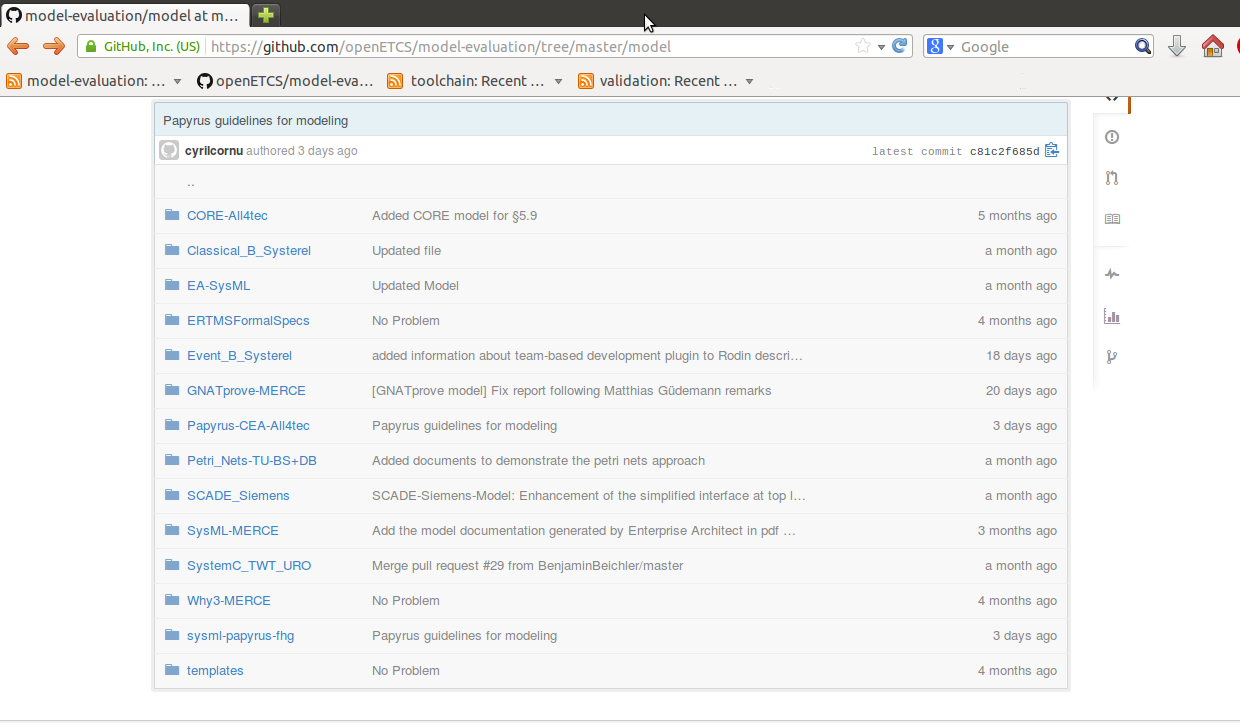
\includegraphics[scale=0.35]{images/models.png}}
  \caption{Repository of models}
  \label{fig:models}
\end{figure}


\section{Evaluation results}

In the conclusion part of O7.1.3-O7.1.7 \citep{WP7_O713_O717}, the first table (see \ref{fig:phaseresults}) show how the evaluated approaches cover  the openETCS design process: 

 \begin{figure}
  \centering
\begin{tabular}{|l | c | c | c | c | c | c | c | c | c | c |}
\hline
&  \rotatebox{90}{GOPRR} & \rotatebox{90}{ERTMSFormalSpecs} &  \rotatebox{90}{SysML with Papyrus} &  \rotatebox{90}{SysML with EA} &  \rotatebox{90}{SCADE} &  \rotatebox{90}{EventB} &  \rotatebox{90}{Classical B} &  \rotatebox{90}{System C} & \rotatebox{90}{Petri Nets} &  \rotatebox{90}{GNATprove} \\
\hline 
System Analysis & \textcolor{blue}{5} & 1     & \textcolor{magenta}{7} & \textcolor{red}{\textbf{9}} & 3     & \textcolor{red}{\textbf{9}} & 3     & 2 & \textcolor{red}{\textbf{6(9)}}  & 2 (3) \\
\hline
Sub-system formal design  & \textcolor{red}{\textbf{9}} & \textcolor{red}{\textbf{9}} & \textcolor{blue}{6} & \textcolor{magenta}{7} & \textcolor{red}{\textbf{9}} & \textcolor{red}{\textbf{9}} & \textcolor{blue}{5} & \textcolor{blue}{5}  & \textcolor{red}{\textbf{6(9)}}   & 3 (4) \\
\hline
Software design  & \textcolor{red}{\textbf{9}} & \textcolor{green}{0} & \textcolor{blue}{6} & \textcolor{magenta}{7} & \textcolor{red}{\textbf{9}} & \textcolor{blue}{6} & \textcolor{red}{\textbf{9}} & \textcolor{red}{\textbf{9}} & \textcolor{red}{\textbf{6(9)}}   & \textcolor{red}{\textbf{6(9)}}  \\
\hline
Software code generation  & \textcolor{red}{\textbf{9}} & \textcolor{green}{0} & 3     & 3     & \textcolor{red}{\textbf{9}} & 3     & \textcolor{red}{\textbf{9}} & \textcolor{blue}{6} & 2 (3) & \textcolor{red}{\textbf{6(9)}}   \\
\hline
\end{tabular}
  \caption{Use of the approaches during process phases}
  \label{fig:phaseresults}
\end{figure}

The highest score is 9 and means that the criteria is fully respected, the lowest score is 0. The higher scores (more than 6) for each approach is graphically  represented on figure \ref{fig:results}.

 \begin{figure}
  \centering
  \fbox{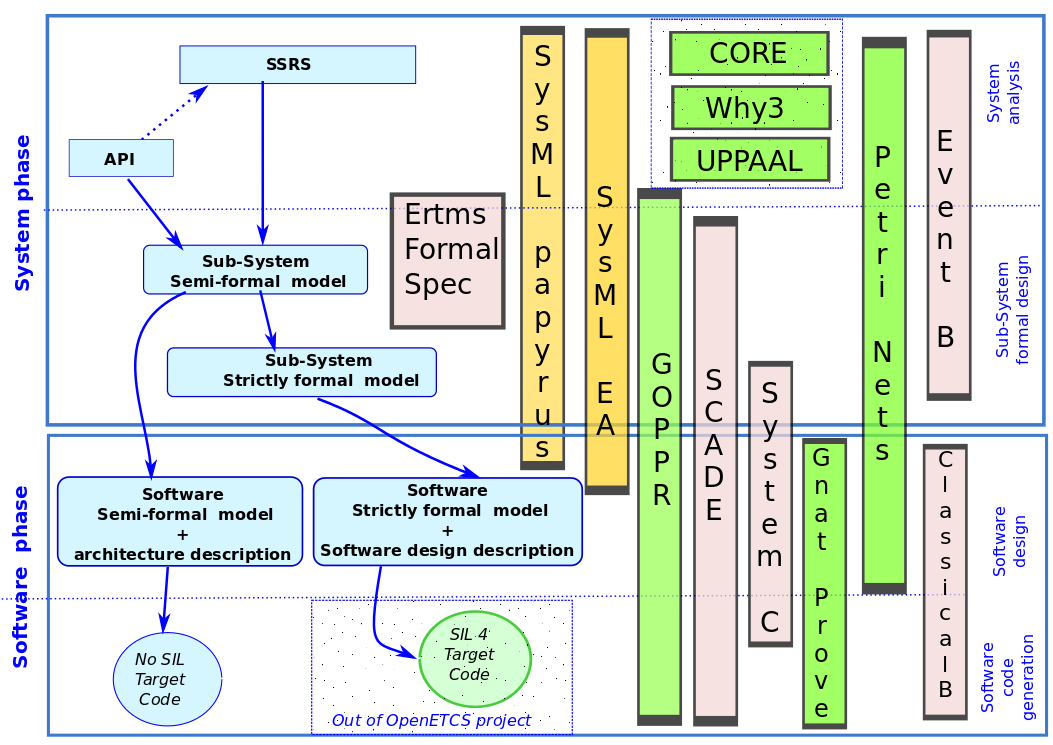
\includegraphics[scale=0.45]{images/First.png}}
  \caption{Results of candidates}
  \label{fig:results}
\end{figure}

The second table (see \ref{fig:activities}) in the conclusion part of O7.1.3-O7.1.7 \citep{WP7_O713_O717}, shows that all evaluated approaches, except GnatProve, are adapted to modeling and design activities:

 \begin{figure}
  \centering
\begin{tabular}{|l | c | c | c | c | c | c | c | c | c | c |}
\hline
& \rotatebox{90}{GOPRR} & \rotatebox{90}{ERTMSFormalSpecs} &  \rotatebox{90}{SysML with Papyrus} &  \rotatebox{90}{SysML with EA} &  \rotatebox{90}{SCADE} &  \rotatebox{90}{EventB} &  \rotatebox{90}{Classical B} &  \rotatebox{90}{System C} & \rotatebox{90}{Petri Nets} &  \rotatebox{90}{GNATprove} \\
\hline 
Documentation & 3     & \textcolor{magenta}{7} & \textcolor{blue}{6} & \textcolor{magenta}{7} & \textcolor{magenta}{8} & \textcolor{magenta}{7} & \textcolor{green}{0} & \textcolor{green}{0} & 2 (3) & 2 (3) \\
\hline
Modeling & \textcolor{red}{\textbf{9}} & \textcolor{red}{\textbf{9}} & \textcolor{red}{\textbf{9}} & \textcolor{red}{\textbf{9}} & \textcolor{red}{\textbf{9}} & \textcolor{red}{\textbf{9}} & \textcolor{red}{\textbf{9}} & \textcolor{magenta}{8} & \textcolor{red}{\textbf{6(9)}}  & 2 (3) \\
\hline
Design  & \textcolor{blue}{6} & \textcolor{red}{\textbf{9}} & \textcolor{blue}{6} & \textcolor{magenta}{7} & \textcolor{red}{\textbf{9}} & \textcolor{magenta}{7} & \textcolor{magenta}{8} & \textcolor{red}{\textbf{9}} & \textcolor{magenta}{5(7)}  & 3 (4) \\
\hline
Code generation  & \textcolor{red}{\textbf{9}} & 1     & 3     & 4     & \textcolor{red}{\textbf{9}} & 3     & \textcolor{red}{\textbf{9}} & \textcolor{blue}{5} * & 2 (3) & \textcolor{red}{\textbf{6(9)}}  \\
\hline
Verification  & \textcolor{green}{0} & \textcolor{magenta}{7} & \textcolor{blue}{6} & 3     & \textcolor{magenta}{8} & \textcolor{red}{\textbf{9}} & \textcolor{red}{\textbf{9}} & 4    * & \textcolor{red}{\textbf{6(9)}}  & \textcolor{red}{\textbf{6(9)}}  \\
\hline
Validation  & \textcolor{green}{0} & \textcolor{red}{\textbf{9}} & \textcolor{blue}{5} & 4     & \textcolor{magenta}{8} & \textcolor{red}{\textbf{9}} & 4     & \textcolor{magenta}{7} & \textcolor{red}{\textbf{6(9)}}  & \textcolor{red}{\textbf{6(9)}}  \\
\hline
Safety analyses  & \textcolor{green}{0} & \textcolor{green}{0} & 4    * & \textcolor{blue}{6} & 1     & \textcolor{blue}{6} & 3     & 3    * & \textcolor{magenta}{5(7)}  &  2(3) \\
\hline
\end{tabular}
  \caption{Use of the approaches according activities}
  \label{fig:activities}
\end{figure}

\section{Short list}

The evaluation process has not been completed for three approaches:

\begin{description}
\item[CORE] The tool is not open source and difficult to obtain, it seems possible to cover the same task with an open-source approach as SysML
\item[Why3] Gnat-Prove covers at least the same service and seems more efficient
\item[UPPAAL] It is a tool dedicated to the verification and validation of time-constraints properties, for example joined with SystemC. It has been proposed for the benchmark on secondary tools (T7.2).
\end{description}

At the end of the evaluation, three others approaches have been discard from the primary tool chain :

\begin{description}
\item[GOPPR] SysML seems a better candidate to offer the same services.
\item[GnatProve] According the results (see \ref{fig:activities}), GantProve has been proposed to joined the evaluation of secondary tools (task T7.2).
\item[PetriNets] However it is a well-known formal approaches, more recent approaches seems more adapted to the goals of the project.
\end{description}

Two tools associated to the SysML approach have been proposed to the evaluation: Papyrus and Enterprise Architect. After discussion on pros and cons of each, partners agree that Papyrus covers better the objectives of the project, especially the open-source requirement. 

Due to the evaluation and discussion during the decision meeting, the partners agreed on a short-list of approaches (see \ref{fig:short_list}):


\begin{enumerate}
\item  ERTMSFormalSpecs
\item  SysML with Papyrus
\item  SCADE
\item  EventB with Rodin
\item  Classical B with Atelier B
\item  System C
\end{enumerate}
 
 \begin{figure}
  \centering
  \fbox{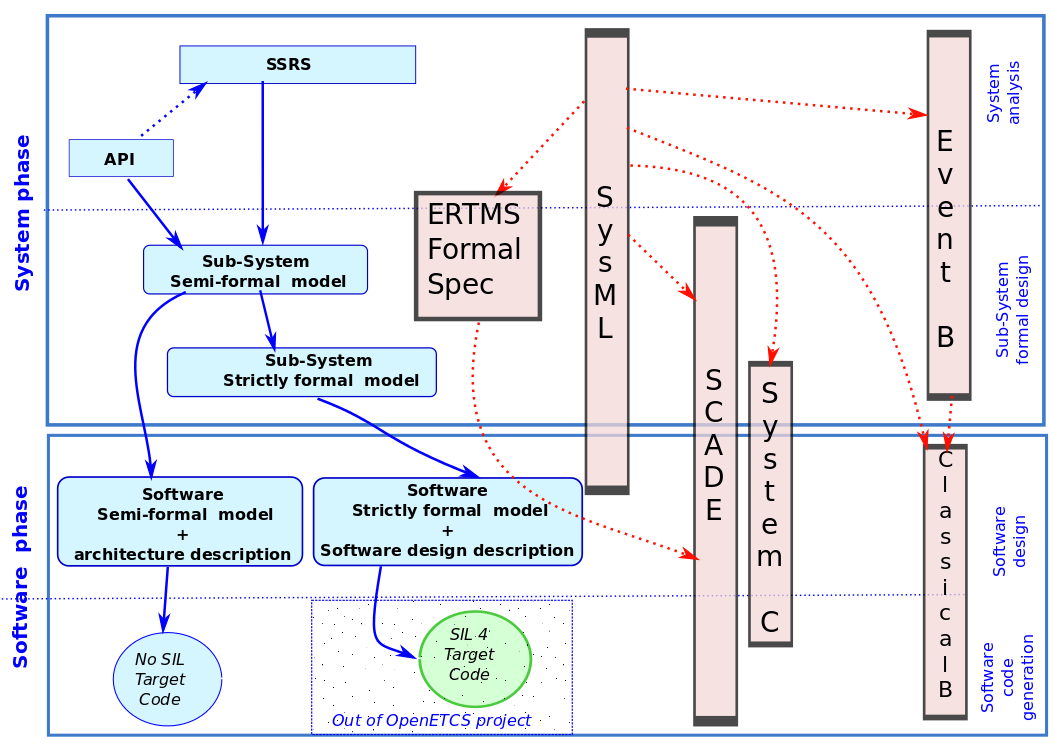
\includegraphics[scale=0.45]{images/Interaction.png}}
  \caption{Short list of candidates}
  \label{fig:short_list}
\end{figure}

